\subsection{\large{\textit{tI}16-CoSiCu\textsubscript{2}S\textsubscript{4} (Direct)}}\vspace{-0.1in}
Cobalt Copper Silicon Sulfide


\begin{figure}[H]
\begin{minipage}{0.34\textwidth}\centering
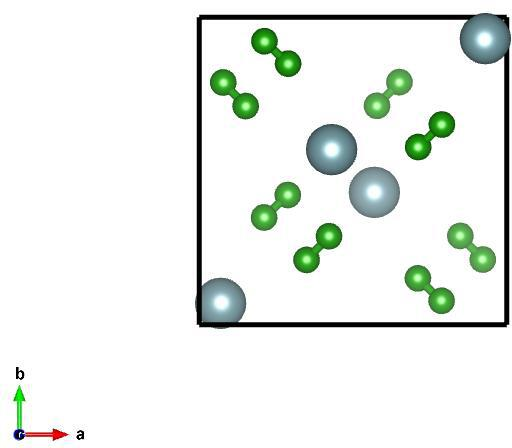
\includegraphics[width=0.9\linewidth,height=2in,keepaspectratio]{/Users/rosecers/work_folders/structures_for_photonics/reference/ref_inp/workspace/0a3749423862c53120b3f24439272c7e/final_images/analog_trim.jpg}\\
\small{Image of \textit{tI}16-CoSiCu\textsubscript{2}S\textsubscript{4}, generated by Vesta}
\end{minipage}\hfill
\begin{minipage}{0.65\textwidth}\raggedright
{\setlength{\mathindent}{0cm}
\begin{equation*}
\begin{split}&\boldsymbol{a_1} = -0.4138049235\ \hat{x} + 0.4138049235\ \hat{y} + 0.8108828341\ \hat{z}\\[-8pt]
&\boldsymbol{a_2} = 0.4138049235\ \hat{x} - 0.4138049235\ \hat{y} + 0.8108828341\ \hat{z}\\[-8pt]
&\boldsymbol{a_3} = 0.4138049235\ \hat{x} + 0.4138049235\ \hat{y} - 0.8108828341\ \hat{z}
\end{split}
\end{equation*}}

\textbf{Space Group:}	121\hspace{0.5in}\textbf{Point Group:}	$\bar{4}2m$\\
\textbf{Crystallographic Open Database} \#1533601\\
\textbf{Structure DOI: }\url{10.1016/j.jallcom.2004.02.004}

\end{minipage}\hfill
\end{figure}
\vspace{-0.25in}


\begin{figure}[H]
\begin{minipage}{0.9\textwidth}\centering
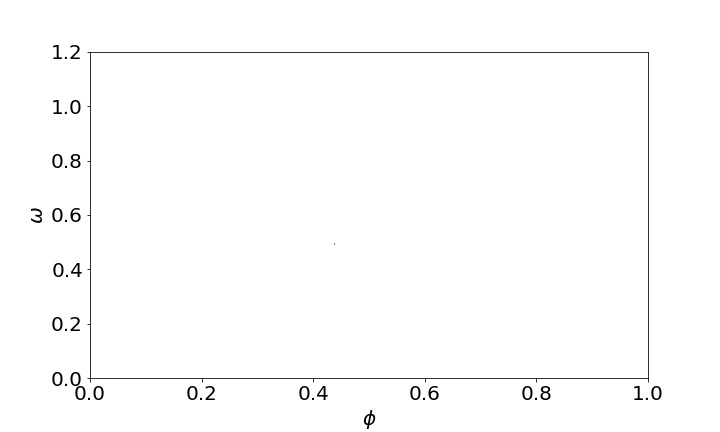
\includegraphics[width=0.9\linewidth,height=2.5in,keepaspectratio]{/Users/rosecers/work_folders/structures_for_photonics/reference/ref_inp/workspace/0a3749423862c53120b3f24439272c7e/final_images/gap_atlas.jpg}
\\
\end{minipage}\hfill\caption{Gap Atlas across filling fraction $\phi$ and frequency $\omega$}
\end{figure}


\begin{figure}[H]
\begin{minipage}{0.5\textwidth}\centering
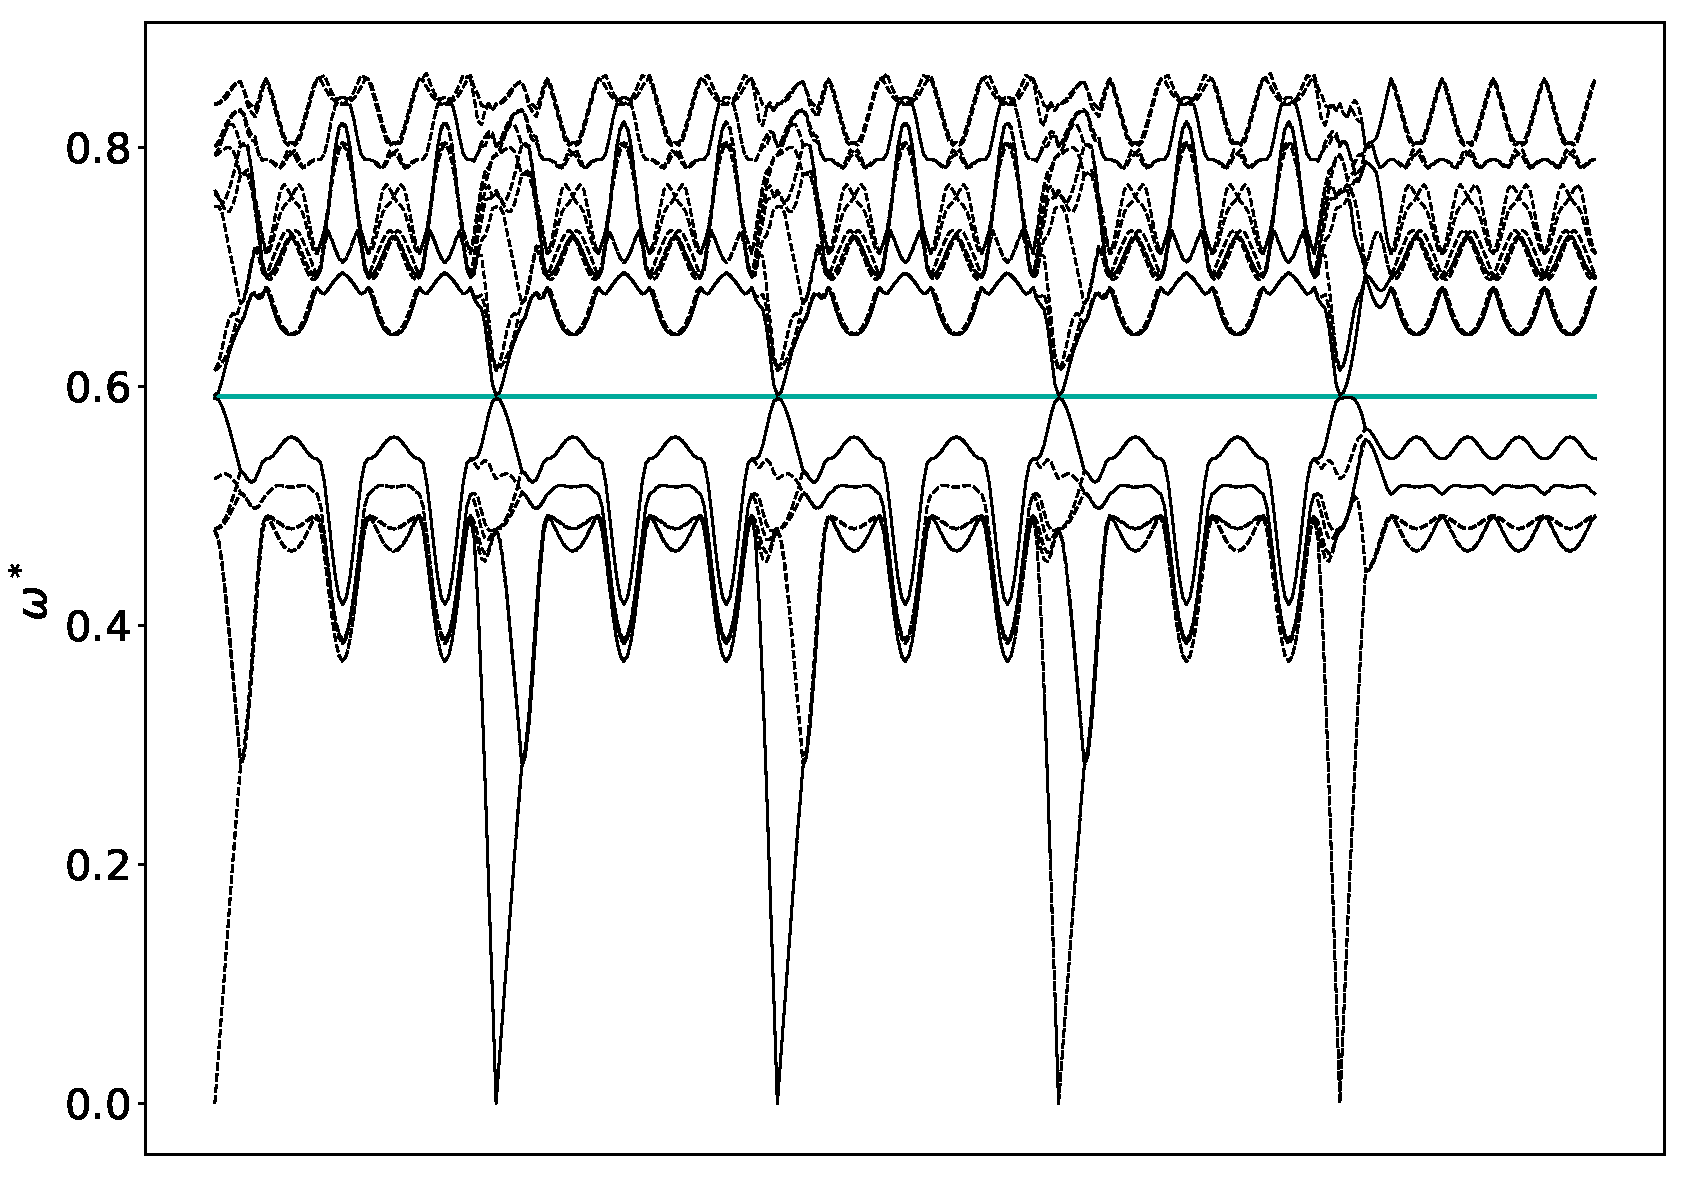
\includegraphics[width=0.9\linewidth,height=1.5in,keepaspectratio]{/Users/rosecers/work_folders/structures_for_photonics/reference/ref_inp/workspace/0a3749423862c53120b3f24439272c7e/./final_images/band_diagram_b=8.pdf}
\\Band Structure across 1st BZ
\end{minipage}\hfill
\begin{minipage}{0.48\textwidth}\centering
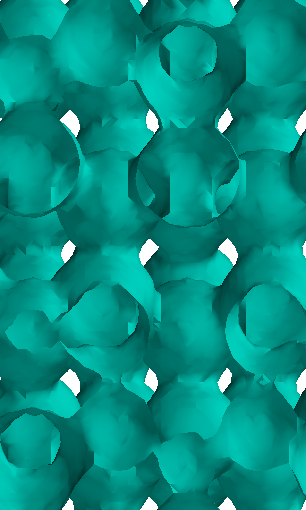
\includegraphics[width=0.9\linewidth,height=1.5in,keepaspectratio]{/Users/rosecers/work_folders/structures_for_photonics/reference/ref_inp/workspace/0a3749423862c53120b3f24439272c7e/final_images/tI16-CoSiCu2S4@gap_8-9.png}
\\View along $a_1$ 
\end{minipage}\hfill\caption{Band Structure and Isosurface of \textit{tI}16-CoSiCu\textsubscript{2}S\textsubscript{4} (Direct) at radius = 0.2, filling fraction = 0.465, where the largest gap between bands 8 and 9 occurs with gap size 12.26\%.}

\end{figure}
\vspace{-0.25in}

